\section{Applikationslaget}
Applikationslagets formål er at skabe en platform for en bruger, så der ikke bemærkes hvad der foregår i de underliggende lag, men skaber en illusion om en direkte forbindelse mellem to applikationslag.
\newline
I dette afsnit gives teorien bag persistens og beskrivelse af de klasser som bruges i applikationslaget. Desuden er der en gennemgang af appilkationens user interface.

\subsection{Teori om persistens}
Persistens er en problemstilling, der skal tages højde for, når man gerne vil bruge data mellem forskellige instanser af en applikation. For at  kalde din data persistent skal man også kunne få adgang til dataen, selvom at applikationen har været lukket ned i mellemtiden. For at kunne lave dataen persistent skal man først bestemme sig for, hvordan man vil gemme sin data. Dette kan gøres på forskellige måder, så som at gemme det i filer eller gemme det på en database. For at kunne aflæse dataen nemt, skal der opstilles retningslinjer for din data. Dette kunne for eksempel være, at hver gang der gemmes noget nyt i en fil, skal der være på en ny linje\cite{oosa}.

\subsection{Controller klassen}
Der blev valgt at samle programmets vigtigste funktioner i klassen \texttt{Controller}. Dette blev gjort for at user interface kun skulle i kontakt med én klasse og fordi det ville blive nemmere i en senere iteration at implementere et Grafisk User Interface (GUI).

\subsubsection{Afsending af besked}
En af controller klassens funktioner er at sende en besked. Denne funktionalitet har fået navnet \texttt{sendBesked(besked, uName)}. Samarbejdsdiagrammet for \texttt{sendBesked()} er vist i figur \ref{fig:sdsend}
\begin{figure}[ht]
	\centering
	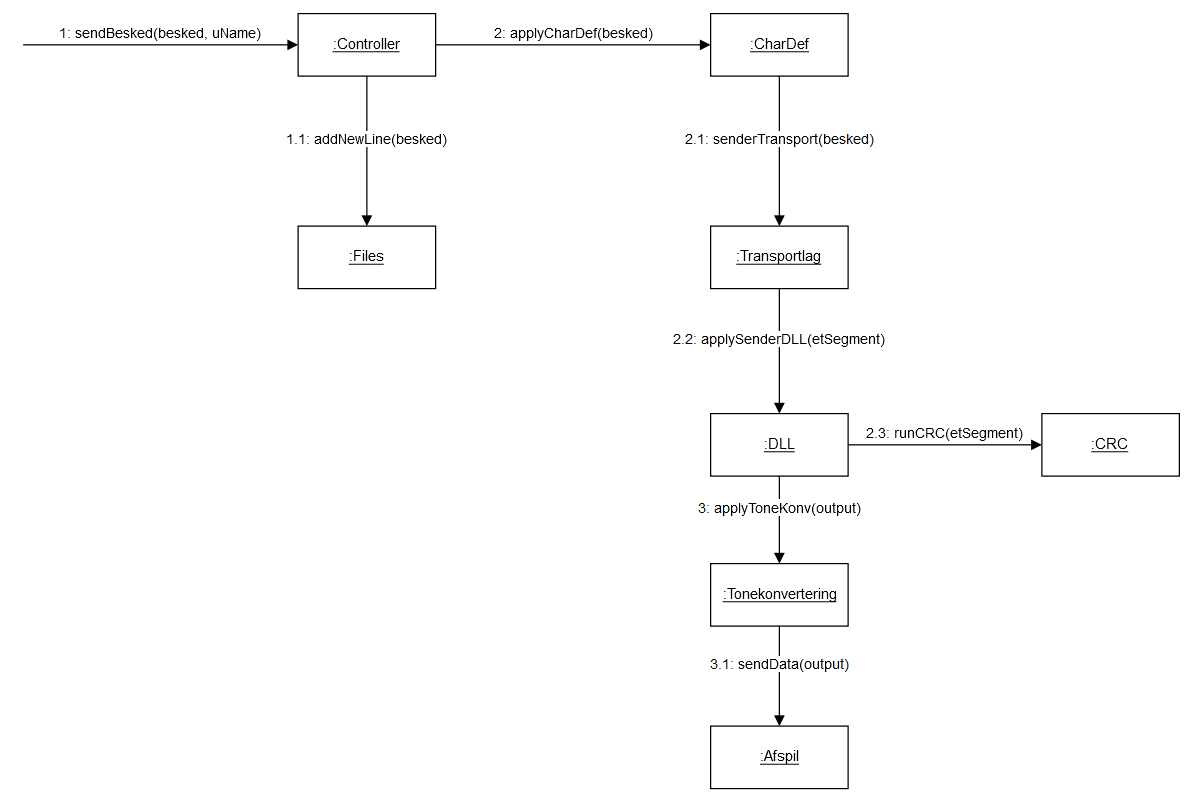
\includegraphics[width=15cm,height=25cm,keepaspectratio]{pictures/SDsend.png}
	\caption{Samarbejdsdiagram for \texttt{sendBesked()}}
	\label{fig:sdsend}
\end{figure}
\newline
\texttt{sendBesked()} tager beskeden der skal sendes, samt navnet på den der har sendt den, og samler det i en besked. Denne besked bliver sendt videre til \texttt{Chardefinition} klassen, som laver teksten om til en binær streng. Den bliver efterfølgende sendt til transportlaget, der kan dele beskeden op i mindre segmenter, der sørger for at beskederne sendes pålideligt. Pakkerne kommer videre til Data Link Laget, hvor der vil blive tilføjet CRC og stuffing til bitstrengen. I \texttt{Tonekonvertering} bliver den binære streng omdannet til tal mellem 0 og 15, som svare til de toner vi har til rådighed, disse toner hedder DTMF. Til sidst bliver tonerne afspillet med klassen \texttt{Afspil}. Når en besked er sendt, bliver den gemt i en fil med klassen \texttt{Files}. Hvis der under dette forløb sker en fejl, bliver der sendt en fejlbesked retur til controlleren.

\subsubsection{Modtagelse af besked}
\texttt{Controller} klassen har desuen en metode til at modtage beskeder. Denne metode hedder \texttt{modtagBesked(uName)}. Samarbejdsdiagrammet for \texttt{modtagBesked()} er vist i figur \ref{fig:sdmod}
\begin{figure}[ht]
	\centering
	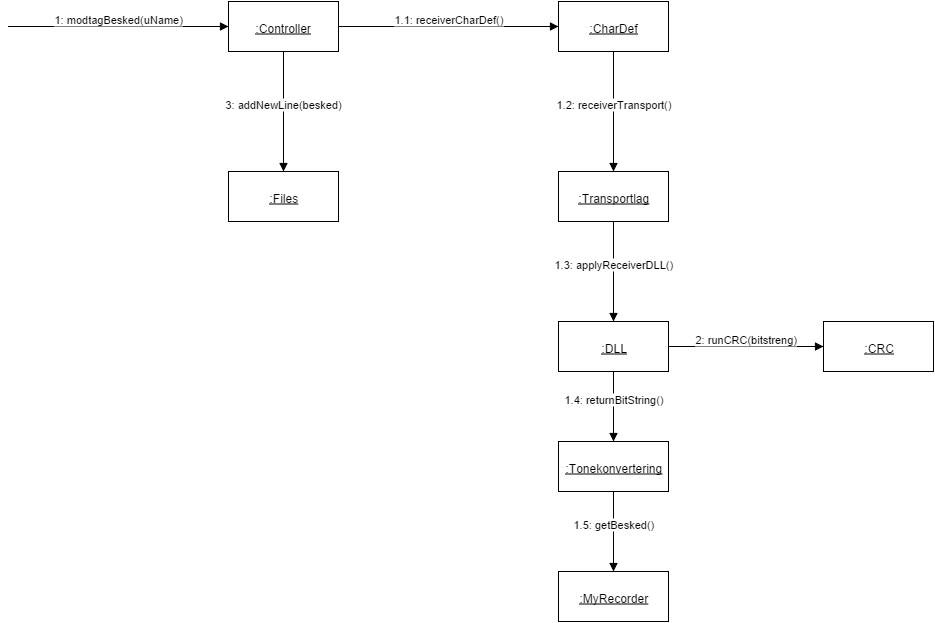
\includegraphics[width=15cm,height=25cm,keepaspectratio]{pictures/SDmodtagBesked.png}
	\caption{Samarbejdsdiagram for \texttt{modtagBesked()}}
	\label{fig:sdmod}
\end{figure}
\newline
\texttt{modtagBesked()} går igennem de samme klasser som \texttt{sendBesked()}, dog i stedet for at sende en besked afsted, sendes der en request om at modtage en besked. I klassen \texttt{MyRecorder} modtages beskeden, som returnere en vektor af tal, der repræsenterer en tone mellem 0 og 15, til \texttt{Tonekonvertering}en. Her omdannes tonerne til en bitstreng, som returneres til \texttt{DLL} klassen. Ved DLL tjekkes for CRC og stuffing fjernes inden det returneres til Transportlaget, hvor beskeden sammensættes. Den kommer retur til \texttt{CharDef} og bliver lavet fra binær streng til karakterer som returneres til \texttt{Controller}, der ved hjælp af UI viser beskeden på skærmen. Samtidig bruges Files til at gemme beskeden i en historik. Til det bruges brugernavnet i \texttt{sendBesked()} for at gemme i den rigtige historik.

\subsubsection{Øvrige metoder i controller}
\texttt{testLogin(uName, pWord)} er metoden der kan teste om et brugernavn og password er korrekt. Det gør den ved at bruge \texttt{Login} klassen.
\newline
\texttt{createUser(uName, pWord)} bruger igen Login klassen, denne gang til at oprette en bruger.
Der er også metoder der kan vise historikken. Disse metoder bruger alle funktioner fra klassen \texttt{Files} og kan enten vise hele historikken, sidste besked eller en der kan definere hvor mange linjer der skal hentes og vises.

\subsection{Login klassen}
Klassen \texttt{Login} bruges til at oprette og teste en bruger, som har et brugernavn og password.
\newline
Metoden \texttt{addUser(uName, Pword)} opretter nye brugere og gemmer brugernavnet og passwordet i et txt dokument for at opnå persistens. Hvis der allerede er et brugernavn af denne type, fås en besked om at brugeren er taget.
\newline
Klassen har også metoden \texttt{testLogin(uName, pWord)}, som bruger metoden \texttt{validateLogin(uName, pWord)}. Den modtager et brugernavn og password, som bliver lavet om til et login token. Denne token bliver efterfølgende sammenlignet med alle de tokens der er gemt i txt filen. Hvis der findes et match bliver der returneret true og brugeren logges på.

\subsection{Files klassen}
\texttt{Files} klassen bruges til at gemme og tilgå historikken, når der bliver skrevet til hinanden med chat programmet. \texttt{Files} virker ved at når der oprettes et objekt at klassen, med en parameter, som er brugernavnet, bliver der oprettet et tekstdokument med brugerens navn, hvis dette ikke findes, som historikken kan gemmes i. Herefter bruges følgende metoder til at bearbejde historikken:
\begin{itemize}
	\item \texttt{addNewLine(besked)} tilføjer en besked til tekstdokumentet, for at gøre det persistent.
	
	\item \texttt{updateVector()} bruges til at lave en vektor af linjerne fra historikken, som efterfølgende kan bearbejdes.
	
	\item \texttt{printVector()} kan printe hver linje ud, som er i vektoren skabt med \texttt{updateVector()}.
	
	\item \texttt{clearText()} kan slette alt fra historikken.
	
	\item \texttt{printLatest()} printes den sidste besked.
	
	\item \texttt{printLines(startN, endM)} kan printe de valgte linjer ud fra linje n til m.
	
	\item \texttt{flipVector()} bruge til vende vectoren, så f.eks. den sidste modtagne besked kommer til at ligge øverst i vektoren, altså på plads 0.
\end{itemize}

\subsection{CharDefinition klassen}
\texttt{CharDefinition} klassens opgave er at omdanne beskeder til en binær repræsentation som det underlæggende Transportlag kan forstå, og omvendt. Når der oprettes et objekt af klassen, bliver der lavet en liste over alle de tal, karakterer og andre tegn, der er mulighed for at sende.
\newline
Klassen indeholder metoden \texttt{charToBinary(input)} som omdanner indputtet, som er en string af karakterer, til en binær string. Det gør den ved at sammenligne karaktererne, der skal sendes, med dem i listen. Når der findes et match, bruges nummeret på placeringen af karakteren i listen, til at udregne en binær værdi, der bliver repræsenteret, ved hjælp af 8 bits. F.eks. vil karakteren b, som har placeringen 11, få den binære værdi 00001011.
\newline
\texttt{applyCharDef(input)} anvender denne metode og sørger for at den binære repæsentation sendes videre til \texttt{Tranportlaget}.
\newline
\texttt{binaryToChar(messageReceived)} omdanner hvert segment af otte bits om til et decimaltal, der bruges i listen til at finde de modtagne karaktere. Karaktererne sættes på en string indtil hele beskeden er omdannet.
\newline
\texttt{receiverCharDef()} bruger denne metode, når en besked returneres fra \texttt{Transportlaget}. Hvis beskeden der modtages er en fejlbesked sendes den videre og der bruges ikke \texttt{binaryToChar()}.

\subsection{UI source}
Til chat programmet er der valgt at lave et simpelt user interface. Dette blev lavet ved at bruge konsolvinduet i Visual Studio. Et flowdiagram af systemet er vist på figur \ref{fig:uiflow}.
\begin{figure}[ht]
	\centering
	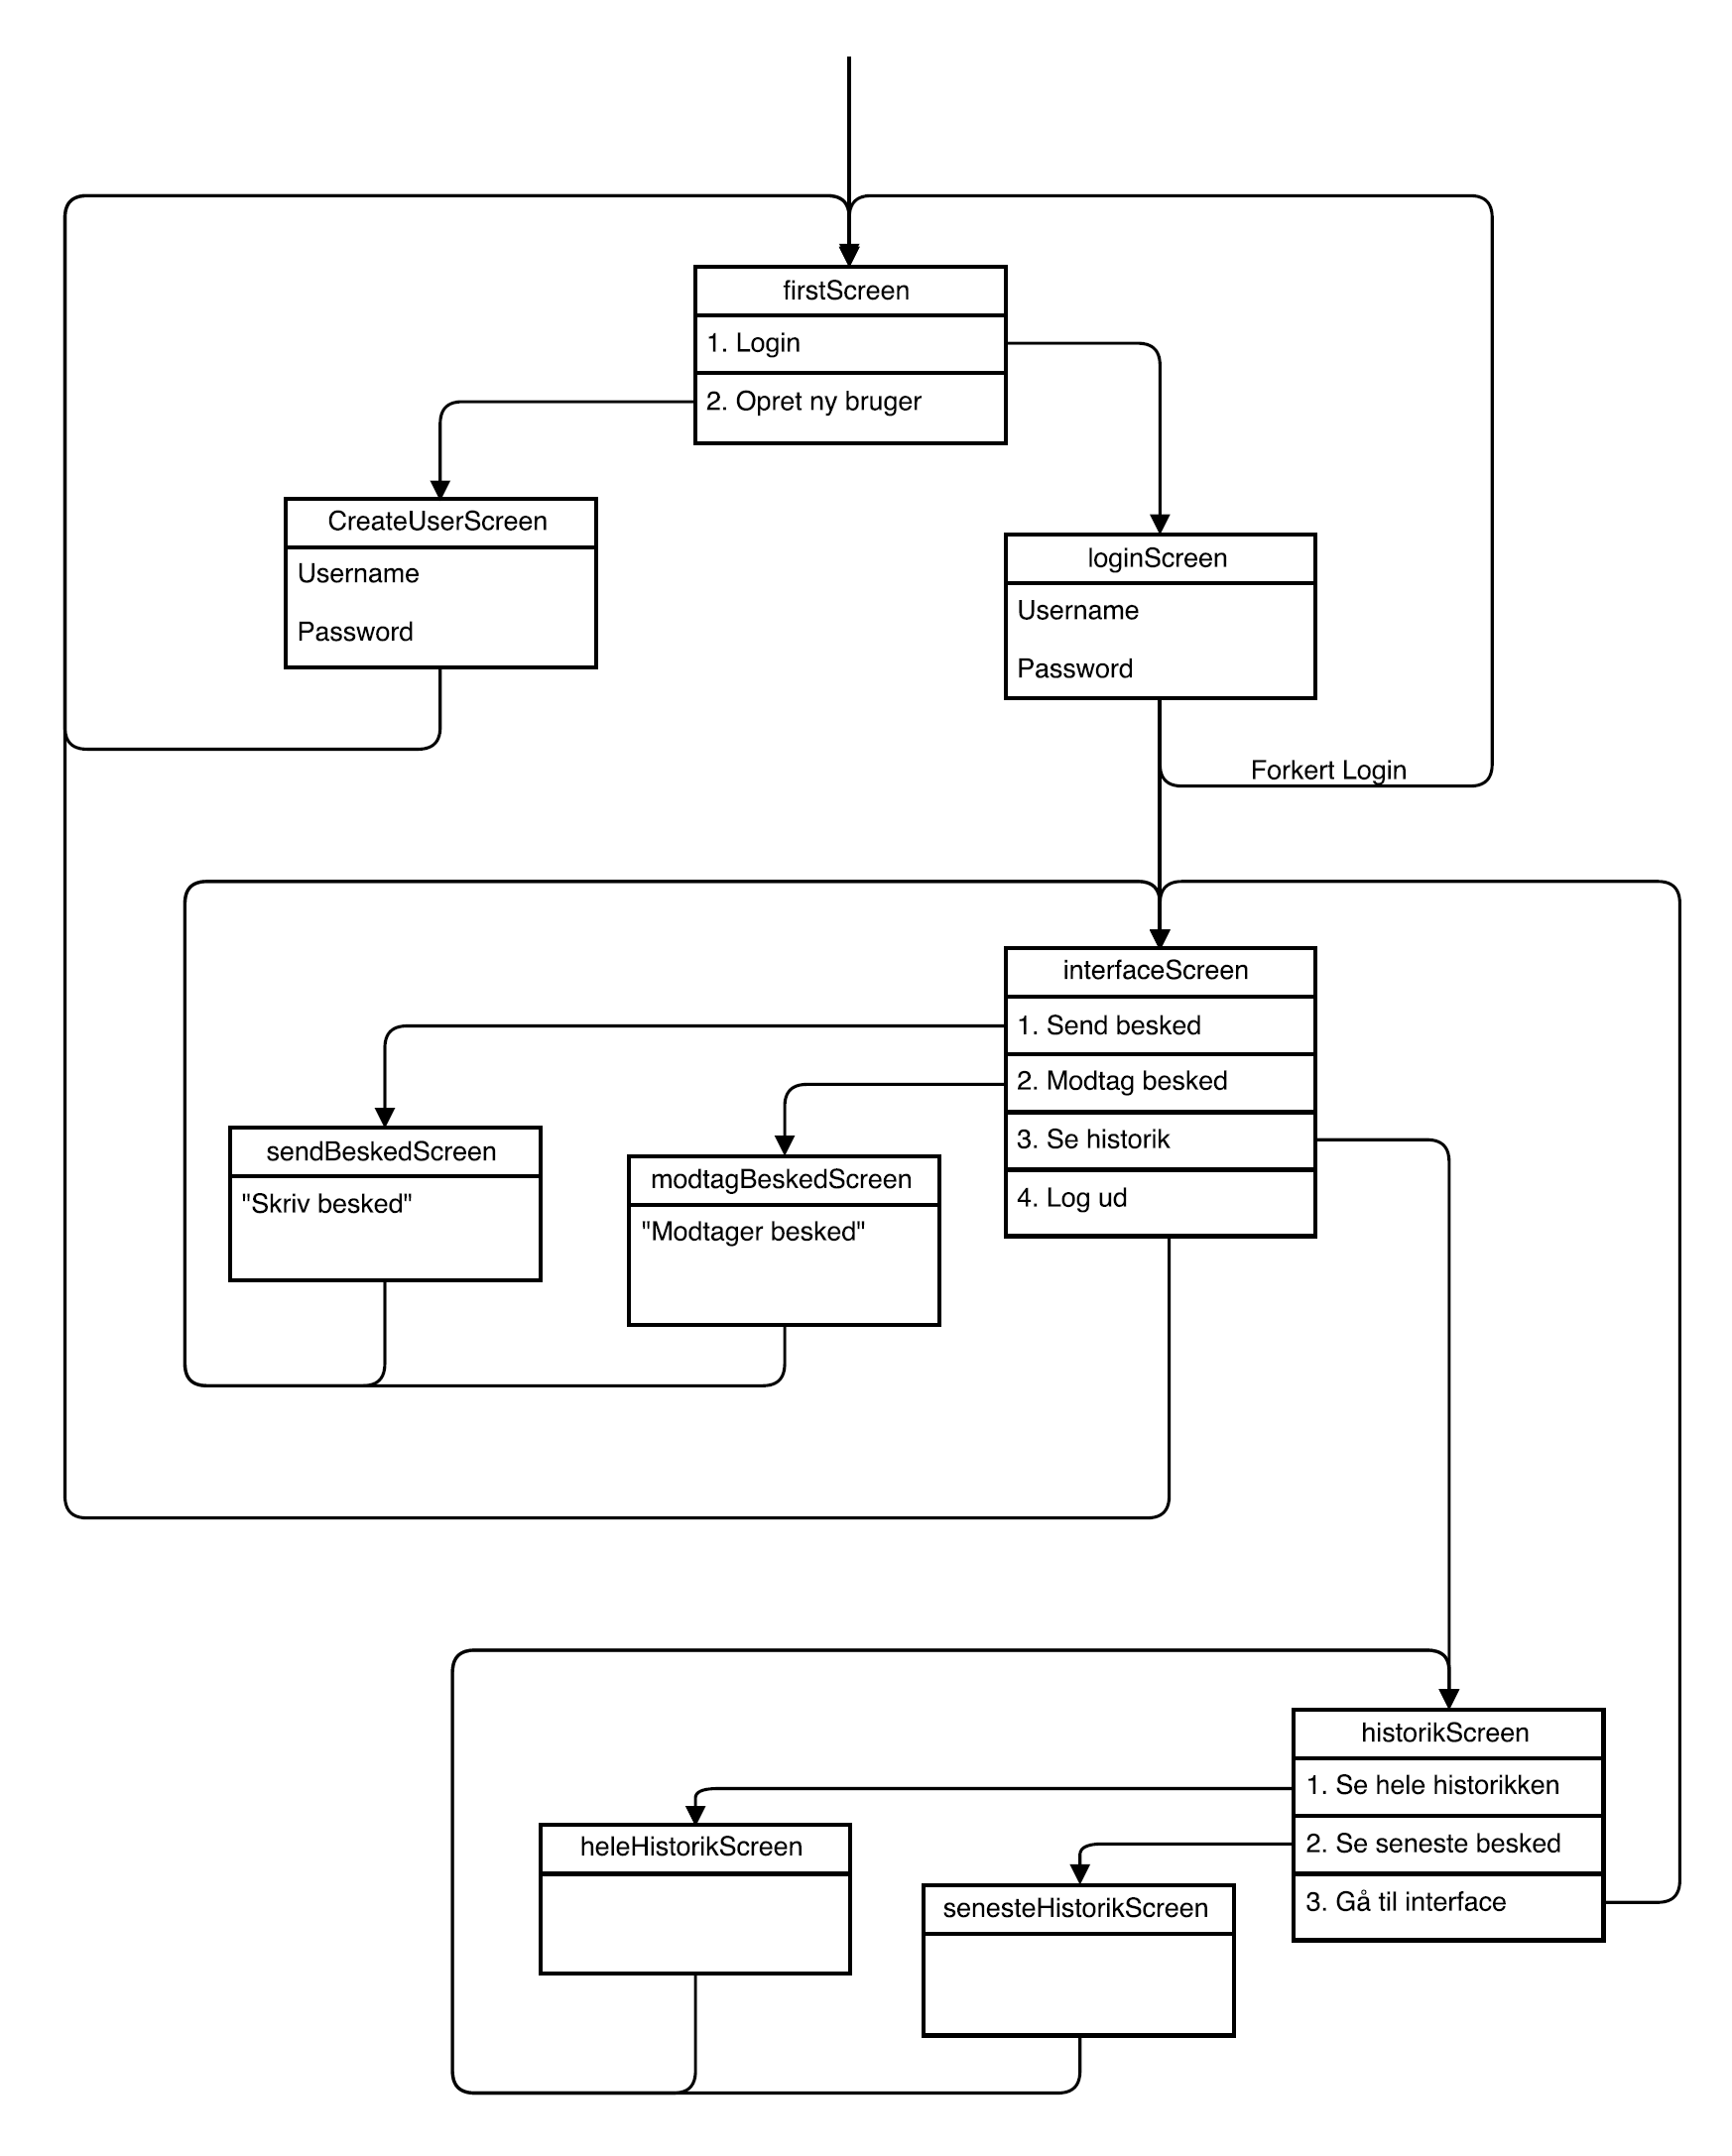
\includegraphics[width=12cm,height=22cm,keepaspectratio]{pictures/UIflow.png}
	\caption{Flowdiagram af UI}
	\label{fig:uiflow}
\end{figure}
Applikationens UI er bygget op ved at der gives nogle valgmuligheder. På første skærm kan der vælges mellem login eller opret bruger. Der vælges ved at indtaste et tal, her 1 eller 2. Tallet sammenlignes med de muligheder der er, og applikationen går til næste skærm.
\newline
Når der oprettes ny bruger, indtastes brugernavn og password som efterfølgende bruges i \texttt{Controller} klassen i metoden \texttt{createUser(uName, pWord)}. Der vil efterfølgende gås videre til loginskærmen, hvor brugernavn og password indtastes igen og bruges i metoden \texttt{testLogin(uName, pWord)}. Hvis det indtastede er forkert kan der prøves igen ellers kommer interface skærmen.
\newline
På interface skærmen er mulighederne:
\begin{itemize}
	\item Send besked
	\item Modtag besked
	\item Se historik 
	\item Log ud
\end{itemize}
Ved "Send besked" skærmen kan der skrives en besked, som efterfølgende sendes med metoden \texttt{sendBesked(besked, uName)} fra \texttt{Controller}. Ved "Modtag besked" skærmen afventes der en besked. Denne modtages med metoden \texttt{modtagBesked()} og bliver efterfølgende vist på skærmen.
\newline
Hvis der vælges historik, kommer en skærm med 3 muligheder igen. Her kan der vælges at se hele historikken eller seneste besked som vises med metoderne \texttt{getHeleHistory()} og \texttt{getSenesteHistory()} fra \texttt{Controller}. Den ved den sidste valgmulighed sendes man retur til interface skærmen, dette kan ses i figur \ref{fig:historik}.
\begin{figure}[ht]
	\centering
	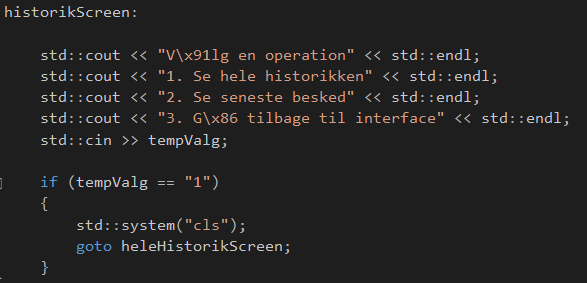
\includegraphics[width=12cm,height=22cm,keepaspectratio]{pictures/historik.PNG}
	\caption{Label historikScreen}
	\label{fig:historik}
\end{figure}
For at kunne holde styre vores UI har vi valgt at bruge kommandoen GOTO som kan springe i mellem labels. For at vælge en af de givne valgmuligheder har vi brugt if sætninger til analysere inputtet fra kommandoen cin